\documentclass[]{thesis-ekf}
\usepackage[T1]{fontenc}
\PassOptionsToPackage{defaults=hu-min}{magyar.ldf}
\usepackage[magyar]{babel}
\usepackage{graphicx,amsmath,amssymb,amsthm,hulipsum, listings}
\footnotestyle{rule=fourth}

\newtheorem{tetel}{Tétel}[chapter]
\newtheorem{lemma}[tetel]{Lemma}
\theoremstyle{definition}
\newtheorem{definicio}[tetel]{Definíció}
\newtheorem{feladat}[tetel]{Feladat}
\theoremstyle{remark}
\newtheorem{megjegyzes}[tetel]{Megjegyzés}
\newtheorem*{megoldas}{Megoldás}

\DeclareMathOperator{\tg}{tg\!}

\lstset{language=[Sharp]C}
\lstset{numbers=left}
\begin{document}
	\logo{
\includegraphics{figures/eszterhazy-logo-hu}}
	\institute{Matematikai és Informatikai Intézet}
	\title{Második beadandó feladat mint szakdolgozat}
	\author{Fügedi Csaba\\ Programtervező informatikus}
	\supervisor{Tanár Neve\\ Beosztása}
	\city{Eger}
	\date{2021}
	\maketitle
	\tableofcontents
	\chapter{Kedvcsináló}
	\section{Bevezetés}
	\textbf{Csillagok Háborúja} \textit{(eredeti cím: Star Wars)} \Az Csillagok háborúja (Star Wars) eredetileg űropera-filmsorozat, amely George Lucas filmrendező ötletein alapszik. A filmek cselekménye a „réges-régen, egy messzi-messzi galaxisban…” élő szereplők történetét meséli el. 
	\textit{\Az első filmet} 1977-ben mutatták be a mozik Csillagok háborúja címmel (1981-ben Egy új remény-re változott a címe), a film gyorsan a popkultúra megkerülhetetlen klasszikusává vált, amely számos más filmre és tudományos-fantasztikus műre volt hatással. Az első filmet két sikeres folytatás követte, az 1980-ban bemutatott A Birodalom visszavág, illetve az 1983-as A Jedi visszatér, ez a három film alkotja az eredeti Star Wars trilógiát. \Az eredeti trilógiát 1999 és 2005 között egy előzmény trilógia követte, amely megosztó reakciókat váltott ki mind a rajongókból, mind a kritikusokból. 2015-ben A Jedi visszatér eseményei után játszódó újabb trilógia vette kezdetét Az ébredő Erő című epizóddal. Az első nyolc film több Oscar-díj jelölést is kapott, ám díjat csak az első két film nyert. \Az filmek hatalmas sikernek bizonyultak, az összes bemutatott film együttvéve 8,5 milliárd dollár bevételt termelt a mozik kasszáinál, ezzel a Star Wars második legjövedelmezőbb filmsorozat a Marvel Cinematic Universe filmjei mögött. Eddig két antológia film készült el, ezek a Zsivány Egyes (2016) és a Solo: Egy Star Wars-történet (2018).
	
	Napjainkra a filmeken kívül könyvek, televíziós sorozatok, számítógépes és videójátékok, témaparki látnivalók, vidámparkok, képregények együttesen birtokolják a Star Wars nevet, ezzel is hozzájárulva a filmek világának fejlődéséhez, bővüléséhez. \Az filmsorozat birtokolja a legsikeresebb filmes merchandising Guinness-rekordját. 2015-ben a Star Wars márka értékét 42 milliárd dollárra becsülték.
	
	\section{Áttekintés}\footnote{Spoiler alert.}
	\Az Csillagok háborúja (angolul: Star Wars) történetét kilenc mozifilm meséli el. Egy sor más animációs film, könyv, képregény és videójáték (valamint néhány, az eredeti sorozathoz lazábban kapcsolódó spin-off-szerű mesefilm) mutatja be bővebben az eredeti filmek által létrehozott kitalált világot.
	
	\Az filmek és a könyvek idegen világokban játszódnak, a fontosabb szereplők egy része – a mellékszereplőknek pedig nagy része – nem ember, hanem idegen fajokba tartozik – vagy éppenséggel droid –, a cselekmény mégis emberi jellegű. A történetben keverednek a racionális alapokon álló sci-fi elemek (forradalmi küzdelem egy elnyomó rendszer ellen, űrhajók, idegen bolygók és lények, a haditechnikai eszközök kiemelt szerepe), valamint a meseszerű, illetve mitikus vonások (emberfeletti hatalommal bíró harcos-tanító rendek, akik a világot összetartó, misztikus jellegű „Erőt” használják; a Jó és a Gonosz örök küzdelme, az egyéni ellenállás lehetősége a kísértő Gonosz ellen, a Legkisebb Fiú győzelme).
	
	Számos kritikus – és a történet szerzőjének – véleménye szerint a sci-fi külsőségek ellenére a Csillagok háborúja valójában közelebb áll a fantasy, valamint a kalandfilm műfajához. Ettől nem függetlenül a filmsorozat sok vonatkozásban hasonlít a mítoszokhoz. George Lucas szerint az volt a szándéka, hogy egy modern mítoszt hozzon létre: nem a tudományos problémák és a Föld vagy az emberiség jövője izgatta, amikor a készítésbe fogott, hanem történeteket, kalandokat akart mesélni, olyasfajtákat, amikért fiatal korában maga is rajongott: westernek, kalandfilmek és kalandregények, képregények és a Flash Gordon című ponyva-sci-fi tévésorozat. 
	
	\Az korszellemtől, amelyben Lucas felnőtt, ez egyáltalán nem volt idegen: a hatvanas-hetvenes évektől kezdve megfigyelhető a természettudományos optimizmus hanyatlása, sőt a tudományellenesség (ez számos okra vezethető vissza, a legnyilvánvalóbb, de közel sem biztosan az egyetlen a hidegháborús korszak légköre, amelyben az emberiség két egymástól rettegve élő frakcióra oszolva a csúcstechnológiás atomfegyverek árnyékában élte életét, amelyek egyszerre garantálták a kétes békét a kölcsönös elrettentés jegyében, illetve a totális világpusztulást, ha az előbbi véletlenül mégse működne). \Az Csillagok háborújával Lucas nemcsak kilúgozta a sci-fi műfajból egyik lényegét, a természettudományok iránti érdeklődést, de tovább is ment: a legelsőként elkészített filmben, amit később Új reménynek címeztek, a gonosz birodalma által elkészített bolygópusztító szuperfegyver, a Halálcsillag képviseli a tudományos-technológiai fejlődés csúcsát, amelytől még a film leggonoszabb szereplője, Darth Vader is undorodik. 
	
	\Az Csillagok háborúja -- már a neve is sugallja -- egy afféle legenda, stílusa egy modern kori ősi mese, egy amerikai mítosz létrehozását célozza meg. \Az történet a valóságtól elrugaszkodott környezet ellenére nagyon is valós, az ember örök harcáról, alapvetően a jóról és a rosszról szól. Ezek miatt a Csillagok háborúja leginkább külsőségeiben tekinthető sci-finek; igazából sokkal inkább hasonlítható a fantasy alkotásokhoz (mint amilyen például A Gyűrűk Ura); ugyanis csupán inkább a valósághoz képest jövőnek tűnő mitikus környezetben játszódik, ahol a különleges, távoli földrészek helyét bolygórendszerek veszik át. Egyik alkotásban sem játszik fontos szerepet a fizikai valóság határainak betartása, legyen szó varázslatról, az Erő használatáról, vagy olyan eszközökről, mint a fénykard. Fő problémája -- Lucas saját meghatározása szerint -- is a jó és rossz általános küzdelme, mint a mesékben és a fantasyban; nem pedig az emberiség jövője, vagy valamilyen tudományos probléma középpontba helyezése. A sci-fi elemeket felhasználó fantasy altípust science fantasy-nak nevezzük és ma már a Star Wars-t is ebbe a kategóriába soroljuk.
	
	Sok Csillagok háborúja-rajongó a filmeket gyerekként látta, és az akkor forradalminak számító különleges effektusok, a filmek fantáziadús képi világa és cselekményvezetése mély nyomot hagytak bennük. A filmek számos eleme -- így például R2-D2 vagy Csubakka alakja, a fénykard, vagy „Az Erő legyen velünk!” kifejezés, vagy a Darth Vader légzőrostélya által kiadott zaj -- vált kultikus emblémává, nem csak az Egyesült Államokban, hanem világszerte, így a magyar közönség számára is. 
	
	\chapter{Filmek}\label{fej-filmek}
	\section{Áttekintés a filmekről}
	\Az filmsorozat kezdődarabját, a Csillagok háborúját 1977.~ május 25-én mutatták be, majd ezt követően elkészült két folytatása, A Birodalom visszavág (1980. május 21.), majd A Jedi visszatér (1983. május 25.) is.
	
	\cite{cimke}\Az első rész bemutatásának huszadik évfordulójára 1997-ben a IV.~-VI.~ epizódokat újra megjelentették (először a mozikban, utána VHS kazettán), Special Editions címen. Ekkor ugyanis a technika már lehetővé tette olyan speciális effektusok alkalmazását is, amelyek a filmek forgatásának idején még nem voltak lehetségesek. A film feljavításán kívül George Lucas néhány effektust digitálisan újra feldolgozott (digitális Jabba és egy kicsiny, de fontos javítás a Han Solo és Greedo közti harcot bemutató filmrészletben). Ezenkívül 2004.~ szeptember 21-én ismét megjelent az eredeti trilógiának egy újabb kiadása, amelyben szintén találhatunk néhány változtatást. A legjelentősebb és legvitatottabb változtatás az volt, amikor a Csillagok háborúja VI: \Az jedi visszatér című rész utolsó jelenetében Lucas lecserélte az Anakin Skywalkert játszó Sebastian Shaw alakját Hayden Christensenére.
	
	1999-ben került mozikba a rajongók által várva-várt epizód a Star Wars I.~ rész -- Baljós árnyak, mely az eredeti trilógia cselekménye előtt 32 évvel játszódik. Ezt követte további két folytatás, a Star Wars II.~ rész -- A klónok támadása (2002) és a Star Wars III.~ rész -- A Sith-ek bosszúja (2005).
	
	2011-ben megjelent a hat film bluray kiadása, amely szintén tartalmazott kisebb módosításokat, a klasszikus és az előzménytrilógiában egyaránt (utóbbiban például az I.~ rész Yoda-bábfiguráját számítógépes grafikára cserélték).
	
	2012-ben a Disney felvásárolta a Lucasfilmet, amely a sorozat jogaival rendelkezett, majd 2013 májusában Kathleen Kennedy, a Lucasfilm elnöke bejelentette, hogy a következő Star Wars-filmet -- a sorozat hetedik részét, Az ébredő Erőt -- 2014-ben kezdik forgatni J. J. Abrams irányításával (a VII.~ rész forgatókönyvét a rendező Lawrence Kasdan, valamint Michael Arndt írta), a filmet 2015 decemberében mutattak be a mozikban. A folytatás trilógia második részét a Rian Johnson által írt és rendezett Az utolsó Jediket 2017 decemberében mutatták be a mozik. A trilógia befejező epizódját, a Skywalker kora című filmet J. J. Abrams rendezte, 2019 decemberében került a mozikba.
	\section{Cselekmény}
	\begin{figure}	
		\centering
		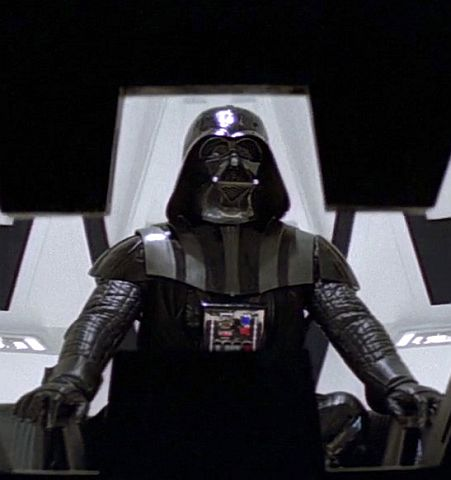
\includegraphics[width=5cm]{figures/dv}
		\caption{Darth Vader, \az{\cite[39. oldal]{cimke}}-hoz hűen}
		\label{fig-dw}
	\end{figure}
	\Az folytatás trilógiával egy időben a Lucasfilm bejelentette, hogy Az ébredő Erő bemutatása után évente olyan új filmek kerülnének a mozikba, melyek már nem a Skywalker-sorozat folytatásai lennének, hanem a Star Wars-univerzum egy-egy hősének története kerülne a filmek középpontjába. Az első ilyen önálló film a 2016 decemberében bemutatott Zsivány Egyes volt, amely a III.~ és a IV.~ epizód között játszódik. Ezt követte 2018 májusában a Ron Howard által rendezett Solo, amely Han Solo fiatalkorát mutatja be. 	
	
	\Aref{fej-konyv}. (\pageref{fej-filmek}.~oldal) fejezetben csak azért ez a téma, mert éppen ez a film megy a háttérben. 
	
	\section{Minden más, ami kell}
	Többszintű lista:
	\begin{itemize}
		\item Első szint.
		\begin{itemize}
			\item Második szint.
			\begin{itemize}
				\item Harmadik szint, amiben van egy gondolatjel -- épp itt -- azért, hogy semmi ki ne maradjon.
			\end{itemize}
		\end{itemize}
	\end{itemize}
	\begin{equation}\label{m-kepl}
		g: \mathbb{R}\setminus \left\{ \mathcal{\mathrm{n}\pi}:\mathcal{\mathrm{n}\in \mathbb{Z}} \right\}\longrightarrow \mathbb{R},  g(x) :=  \left\{ \begin{array}{cl}
			\frac{\mathrm{ctg}_{}^{3}(x)\sin(2x)}{x-1} \text{, ha x > 1}\\
			x(\frac{\mathrm{x}_{}^{2}}{2}+1), \text{ különben.}
		\end{array} \right.
	\end{equation} 
	
	\eqref{m-kepl} képlet a feladatokból.
	
	Random kódrészlet: 
	\lstinputlisting{kod.txt}
	\begin{definicio}\label{def-definition}
		Definíciónak nevezzük általában egy fogalomnak vagy egy jel (például egy nyelvi kifejezés) jelentésének meghatározását.
	\end{definicio}
	\Az{\ref{def-definition}}.~definíció kiegészítése: A filozófiában, logikában, és általában a tudományokban, a definíció avagy meghatározás szót ennél szűkebb értelemben használjuk, a felhasznált szakkifejezések és fogalmak tudományos igényű meghatározását értjük definíción. A legszigorúbb igényességgel a matematika lép fel, egy matematikai definíció akkor helyes, ha bármely szóba jövő dolog esetén egyértelműen meghatározott, hogy kielégíti-e a definíciót vagy sem. 
	
	\begin{thebibliography}{1}
		\bibitem{cimke} \textsc{James Ryan}: When did Star Wars become known as A New Hope? -- In A Far Away Galaxy
	\end{thebibliography}
\end{document}